\section{Problem 3}
\label{sec:problem3}

Because the initial and terminal orbits are circular, the radii follow from $v_c=\sqrt{\mu/r}$ with $\mu=1$:
\begin{equation*}
r_1 = \frac{\mu}{v_{c1}^2} = 1, \qquad r_2 = \frac{\mu}{v_{c2}^2} = 4, \qquad R = \frac{r_2}{r_1} = 4
\end{equation*}
The total impulses from Problem 1 are evaluated at $R=4$ in \texttt{problem3.py} (bi-elliptic for $S\in\{2,5,10,11,12,15\}$, as in Problem 1), and the smallest is selected.

\medskip
\programoutput{outputs/problem3.txt}

\begin{equation*}
\boxed{\text{Hohmann transfer}, \qquad \frac{\Delta V}{v_{c1}} = 0.4487}
\end{equation*}

\begin{figure}[H]
\centering
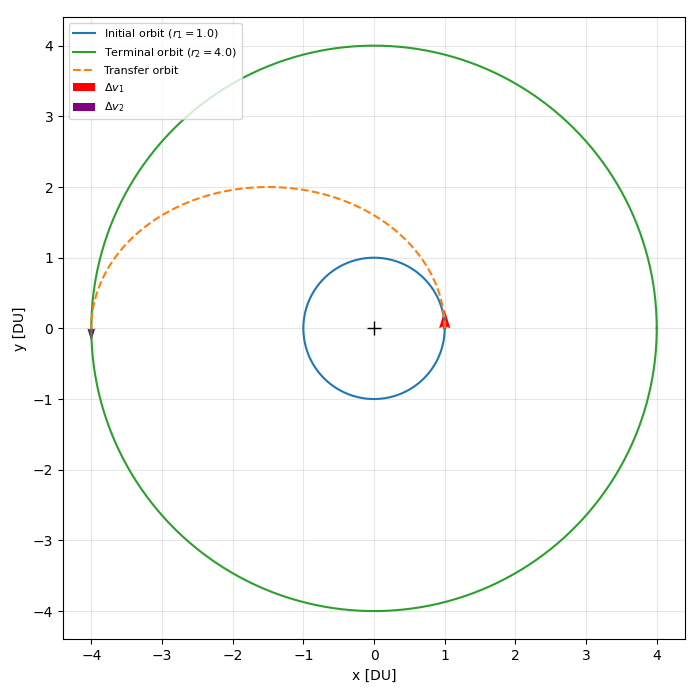
\includegraphics[width=0.65\textwidth]{problem3_transfer.png}
\caption{Hohmann transfer from $r_1=1$ to $r_2=4$ (canonical units), with impulses $\Delta v_1$ and $\Delta v_2$ shown at periapsis and apoapsis of the transfer ellipse.}
\label{fig:p3-transfer}
\end{figure}

\FloatBarrier
